\section{Supervisor}

\frame{\tableofcontents[currentsection]}

\begin{frame}
    \frametitle{Purpose}
    \begin{itemize}
        \item sophisticated error recovery model (99.999999\% uptime)
        \item Process which supervises processes
        \item Fault-tolerance
        \item Failure isolation
        \item Supervision tree
    \end{itemize}
    % \vfill
    % \includegraphics[scale=0.50]{01_supervision_tree}
\end{frame}

\begin{frame}
    \frametitle{Supervision tree}
    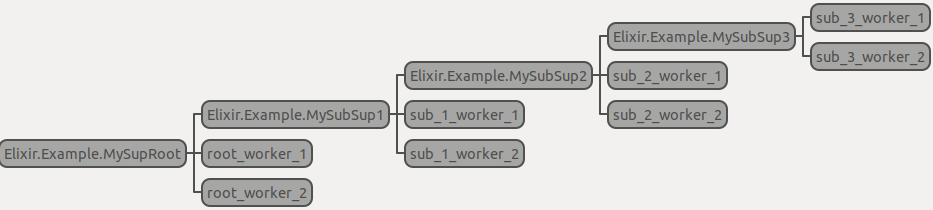
\includegraphics[scale=0.32]{11_supervision_tree}
\end{frame}

\begin{frame}
    \frametitle{Code representation}
    \begin{center}
        \code[language=elixir,font=\scriptsize]{demo-code/basic_supervisor_module.ex}
    \end{center}
\end{frame}

\begin{frame}
    \frametitle{Necessary information}

    \begin{itemize}
        \item How it should start the child.
        \item What it should do when the child terminates.
        \item How it should uniquely distinguish the child.
    \end{itemize}

    \vfill

    \footnotesize
    child specifications and supervisor restart strategy contains this information.
\end{frame}

\begin{frame}
    \frametitle{Rules to be supervised}

    \begin{itemize}
        \item Childs need to be linked
        \item Childs must enforce the shutdown OTP behaviour
    \end{itemize}

    \vfill

    \footnotesize
    If childs do not terminate with reason shutdown, then child is killed with brutal\_kill
\end{frame}